\documentclass[10pt,a4paper]{article}
\usepackage[T1]{fontenc}
\usepackage{lmodern,amsmath,amssymb,booktabs,array,longtable,graphicx,xcolor,tikz,enumitem}
\usepackage[margin=20mm]{geometry}
\usepackage[colorlinks=true,urlcolor=blue,citecolor=blue,linkcolor=blue]{hyperref}
\usetikzlibrary{arrows.meta,positioning}
\setlength{\parindent}{0pt}
\setlength{\parskip}{5pt}
\setlength{\emergencystretch}{2em}
\setlist{nosep,leftmargin=*}
\renewcommand{\arraystretch}{1.17}
\newcommand{\E}{\mathbb{E}}
\newcommand{\R}{\mathbb{R}}
\newcommand{\page}[1]{\clearpage\section{#1}}
\begin{document}
{\Large\bfseries Telemetry-Aware Capacity Elasticity\\in a Three-Stage Service Chain}\par
{\large Mathematical model, independent verification and frozen experiments}\par
Prepared for Fatima Subhi Khaleel\\
\href{mailto:fatima.subhi_eng@uodiyala.edu.iq}{fatima.subhi\_eng@uodiyala.edu.iq}\\
18 October 2026

\textbf{Thesis context:} Optimal Resource Allocation in ORAN with SDN-Managed Orchestration.

\section*{Abstract}
This computational study examines paid capacity elasticity under delayed telemetry
and delayed actuation in a two-class, three-stage packet service chain. A finite-grid
controller combines historical queue extrapolation, a dispersion margin and class
reservations, with local deadline-based borrowing of unused capacity. Strong fixed
comparators are selected using a separate calibration set. An additional locked
evaluation comprises 480 replication/ablation runs and 120 activation-delay runs.
The fresh replication reduces incremental abstract resource cost by
37.77--42.36\% across the three stressed settings relative to the previously selected
fixed expansions. However, prediction is not uniformly helpful, removing the margin
reduces cost while increasing misses, and the nominal case exhibits unnecessary
capacity activation. These findings support a cost--delay trade-off, not universal
policy superiority. Independent packet replay, uncached optimizer enumeration and
37 unit tests verify the implemented abstraction. At a two-second actuation delay,
the dynamic policy loses its cost advantage and has substantially more class-1
misses than fixed expansion. Physical O-RAN validation,
state-of-the-art policy reproduction and a complete novelty review remain open.

\section*{Status and claim boundary}
\textbf{This is a reproducible technical study and manuscript foundation, not a
submission-ready IEEE paper or validated O-RAN result.} No NR physical layer, SDN
protocol, RIC interface or calibrated CPU workload is implemented. All numeric
parameters are synthetic choices. The study does not claim monetary or energy
savings, URLLC guarantees, global optimality, a current Q1 classification or
publication acceptance. No quantum component is included.

\section*{What this release adds}
\begin{itemize}
\item A complete event-order contract, symbols and equations for the implemented model.
\item Correctness propositions with explicit limits and an independent software check.
\item Six controller variants, fresh seeds, command-delay stress tests and paired uncertainty.
\item Negative results, source/parameter provenance and a concrete external-validation gate.
\end{itemize}

\page{Context, closest work and contribution limits}
Open Radio Access Network (O-RAN) exposes architectural interfaces and programmable control opportunities
\cite{polese}. Timestamped telemetry creates an information-age problem rather
than merely a sampling-rate problem \cite{age}. Neither motivation demonstrates
that a particular queue simulator is O-RAN compliant.

Here SDN means Software-Defined Networking, RIC means RAN Intelligent Controller,
NR means New Radio, and URLLC means Ultra-Reliable Low-Latency Communication.
FIFO means first-in, first-out and EDF means earliest-deadline-first. These terms
identify motivations and scheduling concepts, not implemented protocol compliance.

MAREA develops radio-resource allocation around a Martingale-based delay analysis
and multi-timescale control \cite{marea}. The current dispersion score is not a
replacement for its mathematical delay bound. Kalntis et al. study online learning
for virtualized base stations, including a meta-learning mechanism and trace-driven
evaluation \cite{kalntis}. No such learning/regret result is established here.
Joint radio, fronthaul and cloud orchestration is already studied in cell-free
O-RAN \cite{demir}. Therefore ``joint allocation'' alone is not a new contribution.

OREO addresses xApp-based service orchestration and sharing \cite{oreo}, whereas
the present queues represent packet service. Predictive shared AI/RAN orchestration
is also prior art \cite{caora}. These problems are relevant context but not directly
interchangeable benchmark implementations.

\begin{center}\small
\begin{tabular}{p{30mm}p{53mm}p{67mm}}
\toprule
Prior work & Relevant distinction & Consequence for this study\\\midrule
MAREA & Radio delay analysis and two control timescales & Do not claim probabilistic delay guarantees from a queue proxy\\
Adaptive vBS allocation & Online learning and real-world-data evaluation & No claim to beat published learning methods without reproduction\\
Joint cell-free O-RAN & Coupled physical radio/fronthaul/cloud resources & Abstract stages do not demonstrate physical joint optimization\\
OREO & xApp sharing and service deployment & An xApp is not the same object as a packet in this model\\
Predictive AI/RAN & Forecasting and shared compute orchestration & Prediction itself is not a novelty claim\\\bottomrule
\end{tabular}\end{center}

ColO-RAN provides an experimental framework for closed-loop xApps \cite{coloran}.
5G-LENA supplies an end-to-end NR simulation route \cite{lena}, with documented
calibration against reference scenarios \cite{calibration}. Neither was executed
for these results. Their existence identifies a route to external validation,
not a validation certificate for the current code.

\textbf{Potential research question:} How should information refresh and paid
resource elasticity account for pending commands when both sensing and actuation
are delayed? The present experiment explores this interaction but does not yet
establish a substantial novel theoretical or empirical contribution. The three
planned papers cannot be obtained by renaming the same simulation outputs.

\page{System model, units and event order}
Let $i\in\{1,2,3\}$ index stages and $s\in\{0,1\}$ index classes. Time $t$ is
discrete. $A_s(t)$ counts new packets, $Q_{is}(t)$ is the start-of-slot queue before
external arrivals and $S_{is}(t)$ is the number served in that slot. Base capacity
$c_i(t)$ and active expansion $e_i(t)$ are in packets/slot. The evolution is
\begin{align}
Q_{1s}(t+1)&=Q_{1s}(t)+A_s(t)-S_{1s}(t),\\
Q_{is}(t+1)&=Q_{is}(t)-S_{is}(t)+S_{i-1,s}(t),\quad i=2,3.
\end{align}
Stage 1 may serve newly arrived packets. Stages 2 and 3 may serve only packets
present before upstream service in that slot. Each packet consumes one service
unit per stage. Class deadlines are $D_0=15$ and $D_1=40$ slots.

\begin{center}\small
\begin{tabular}{p{53mm}p{98mm}}
\toprule Parameter & Fixed design choice\\\midrule
Slot mapping & 20 ms, synthetic rather than an NR slot\\
Traffic & Poisson rates $(0.9,2.1)$ packets/slot, burst rates $(1.8,3.8)$\\
Burst & $180\le t\bmod600<290$, stressed settings only\\
Base service & $5+\xi$ with $\xi\in\{-1,0,0,1\}$ sampled uniformly by list position\\
Stressed stage & Capacity 3 during $170\le t\bmod600<310$\\
Extra service & Radio-like stage 0, transport/compute-like stages each 0--3\\
Report request interval/history & 5 slots / at most 20 previous slots\\
Report delay/loss & 3 slots and 0.05, or 9 slots and 0.15\\
Activation delay & 10 slots by default, 1--100 in sensitivity study\\
Initial priors & Queue 0, arrivals $(0.9,2.1)$, service $(2.5,2.5)$, variance $(1,1)$\\
Measured cohort & Birth slots 300--3299, simulation through slot 3339\\
Switching coefficient & $\eta=0.25$, abstract cost units\\\bottomrule
\end{tabular}\end{center}

\textbf{Slot order.} Apply due commands, deliver due reports, insert external
arrivals, request a report and compute a new command when $t\bmod5=0$, serve
stages in order 3, 2, 1, update local history and check packet conservation.
The report snapshot is after external arrivals and before service. Loss is
determined by request index. Timestamps refer to measurement time.

\textbf{Local scheduler.} Largest-remainder quotas split $c_i(t)+e_i(t)$ using
$(\alpha,1-\alpha)$. Unused quotas are borrowed by the next queued packet with
earliest absolute deadline. Within-class service is FIFO. This is quota-first
scheduling, not a claim of globally optimal EDF scheduling.

\page{Controller formulation and execution contract}
For the last received report timestamp $\tau_i$, queue $q_{is}$, historical
arrival mean $\lambda_{is}$, service mean $\mu_{is}$ and net-flow variance $v_{is}$,
the activation-time extrapolation and demand proxy are
\begin{align}
\widehat q_{is}(t+L)&=\max\{0,q_{is}+(t+L-\tau_i)(\lambda_{is}-\mu_{is})\},\\
z_{is}&=\widehat q_{is}(t+L)+5\lambda_{is}+\sqrt{(t+L-\tau_i)v_{is}}+1.
\end{align}
The candidate grid is $\mathcal X=\{0\}\times\{0,1,2,3\}^2$ and
$\mathcal A=\{k/20:k=1,\ldots,19\}$. Let $r_{is}(x,\alpha)$ denote integer quotas
from reported base capacity plus candidate expansion. Define
\begin{align}
\rho_s(x,\alpha)&=\frac1{D_s}\sum_{i=1}^{3}\frac{z_{is}}{\max\{0.001,r_{is}(x,\alpha)\}},\\
g(x)&=\sum_i x_i+\eta\sum_i|x_i-x_i^{\rm prev\ request}|.
\end{align}
A candidate with $\rho_{\max}=\max_s\rho_s\le1$ is \emph{surrogate feasible}.
Lexicographic scores are $(0,g,\rho_{\max},\sum_s\rho_s,k)$ if feasible, otherwise
$(1,\rho_{\max},g,\sum_s\rho_s,k)$. All 304 candidates are enumerated. Exact ties
retain the first expansion pair in ascending order.

\begin{center}
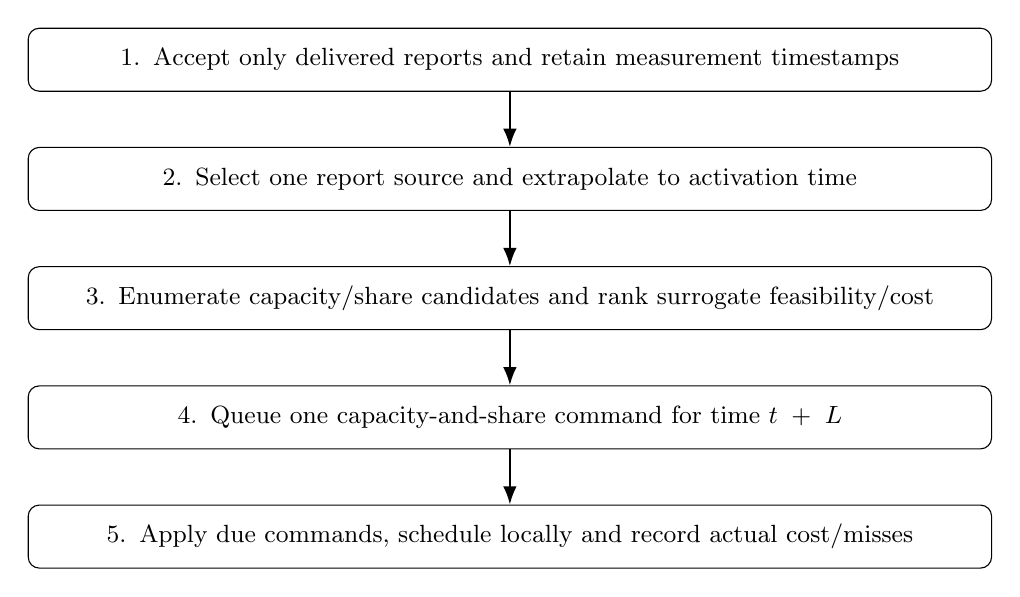
\begin{tikzpicture}[node distance=7mm,box/.style={draw,rounded corners,align=center,text width=120mm,minimum height=8mm,font=\small},arr/.style={-{Latex},thick}]
\node[box] (a) {1. Accept only delivered reports and retain measurement timestamps};
\node[box,below=of a] (b) {2. Select one report source and extrapolate to activation time};
\node[box,below=of b] (c) {3. Enumerate capacity/share candidates and rank surrogate feasibility/cost};
\node[box,below=of c] (d) {4. Queue one capacity-and-share command for time $t+L$};
\node[box,below=of d] (e) {5. Apply due commands, schedule locally and record actual cost/misses};
\draw[arr] (a)--(b);\draw[arr] (b)--(c);\draw[arr] (c)--(d);\draw[arr] (d)--(e);
\end{tikzpicture}
\end{center}

The full telemetry priority is
\[
P_i=\sum_s\frac{\sqrt{(t-\tau_i)v_{is}+1}}{D_s}
\left(1+\frac{\widehat q_{is}(t)}{\max\{1,c_i^{\rm report}\}}\right)+0.01(t-\tau_i).
\]
The maximum is refreshed. The age term is not a starvation proof. The square-root
margin is not statistically calibrated. The 0.001 quota floor is a numerical
penalty, not real service. Commands are not cancelled or coalesced, and the
predictor does not propagate the pending-command pipeline.

\page{Correctness statements and their limits}
\textbf{Proposition 1: packet conservation.} Cumulative generated packets equal
cumulative completed packets plus queued packets at every slot. Summing (1)--(2)
over stages cancels internal transfers. The simulator checks this identity per slot.

\textbf{Proposition 2: work conservation.} Total service at a stage is the minimum
of active capacity and eligible queued packets. Initial quotas cannot overserve
a class. Borrowing uses every remaining unit until either the capacity or all
eligible queues are exhausted. This does not prove deadline feasibility.

\textbf{Proposition 3: minimum packet latency.} For birth slot $b_p$ and completion
slot $f_p$, $f_p-b_p+1\ge3$. The packet must cross three stages and cannot cross
two in one slot. The independent replay also checks this boundary.

\textbf{Proposition 4: finite-grid optimality.} The chosen candidate minimizes
the stated lexicographic score over $\mathcal X\times\mathcal A$. After each
iteration the incumbent is the minimum of the candidates examined so far.
Induction over the finite enumeration proves the statement. It is not continuous
optimality, a stochastic-control theorem or optimality of the total observed cost.

\textbf{Proposition 5: a necessary capacity cut.} All packets born in slots
$[a,b)$ that traverse stage $i$ and have deadlines at most $D_{\max}$ must cross
that stage before their end-to-end deadline. Even granting the enlarged window
$[a,b+D_{\max})$, a necessary condition for zero misses is
\[
\sum_{t=a}^{b-1}\sum_s A_s(t)\le
\sum_{t=a}^{b+D_{\max}-1}\bigl(c_i(t)+e_i(t)\bigr).
\]
Exceeding the right-hand side proves some deadline failures are unavoidable for
those arrivals and capacities. Satisfying the condition does not prove
schedulability. A failed zero-miss condition does not rule out a positive miss target.

\textbf{Complexity.} Direct enumeration is $O(MKIS)$ for $M$ expansion combinations,
$K$ shares, $I$ stages and $S$ classes. Here $(M,K,I,S)=(16,19,3,2)$.
Caching removes repeated stage calculations, but expansion-grid growth remains
exponential if more independently expandable stages are added. No scalability
claim beyond this small model is made.

\textbf{Actual cost.} Across the entire simulation, including warmup and followup,
\[
J=\sum_{t=0}^{T-1}\sum_i e_i(t)+\eta\sum_{t\in\mathcal T_{\rm apply}}
\sum_i|e_i(t)-e_i(t-1)|.
\]
Static capacity is preprovisioned, with no initial switching charge but full
capacity-time cost. The controller's one-decision score $g$ is not $J$. Base
infrastructure costs, power and financial prices are absent.

\page{Evaluation design and statistical interpretation}
The earlier calibration uses seeds 4000--4004 and all 16 fixed capacity pairs.
The cheapest fixed pair whose two calibration mean miss rates are at most 1\%
is selected. The resulting choices are $(0,0)$ for nominal, $(2,0)$ for transport,
$(0,2)$ for compute and $(2,0)$ for delayed/lost transport. The 1\% threshold is
only a comparator-selection rule, not a proven service-level agreement.

The earlier held-out evaluation uses seeds 5000--5019. This release uses a new
local protocol lock, written before seeds 6000--6019 were evaluated. Its SHA-256
is stored with outputs. It is not externally preregistered. Six variants over
four settings and 20 seeds give 480 runs. Six command delays over ten different
seeds 7000--7009 and two policies give 120 additional runs.

\begin{center}\small
\begin{tabular}{p{36mm}p{114mm}}\toprule
Variant & Single controlled difference from full dynamic\\\midrule
Round-robin & Requests rotate through three stages\\
Oldest-first & Requests choose the oldest delivered report\\
No prediction & Uses reported queue directly, still retains the dispersion margin\\
No margin & Removes the square-root term, retains queue extrapolation\\
Selected fixed & Locks capacity at prior calibrated values, retains delayed share control\\\bottomrule
\end{tabular}\end{center}

The measured class rate is the number of late-completed plus unfinished measured
packets divided by all arrivals of that class in the measured cohort. The 40-slot
tail ensures every measured deadline has elapsed. Background arrivals continue
during that tail. Completed-only percentiles are not primary endpoints because
they can hide unfinished packets.

Seed, not packet, is the independent replication unit. Percentile bootstrap
intervals use 10,000 seed-level resamples, pairing policies by seed \cite{efron}.
The intervals are exploratory, especially near zero events. For four settings
and three endpoints, exact paired sign tests omit ties and test whether positive
and negative paired differences are equally likely. All 12 p-values receive
Holm correction as one family \cite{holm}. These tests are not tests of mean
equivalence, noninferiority or an SLA.

If all 20 independent runs have no misses, the exact one-sided 95\% upper bound
on the probability that a new same-distribution run has any miss is
$1-0.05^{1/20}=13.91\%$. This is a run-level statement, not a packet failure
probability. The bound follows from $(1-p)^{20}=0.05$.

\page{Fresh-seed results: all settings and variants}
All values below are seed means for seeds 6000--6019. Miss rates are percentages.
Cost is incremental and abstract. All six variants are retained, including
negative ablation outcomes.
\begin{center}\footnotesize
\begin{tabular}{llrrr}\toprule
Setting & Variant & Class 0 (\%) & Class 1 (\%) & Cost\\\midrule
Nominal & Full dynamic & 0.0000 & 0.0000 & 142.31 \\
Nominal & Round-robin & 0.0000 & 0.0000 & 317.43 \\
Nominal & Oldest-first & 0.0000 & 0.0000 & 281.38 \\
Nominal & No prediction & 0.0000 & 0.0000 & 109.00 \\
Nominal & No margin & 0.0000 & 0.0000 & 0.00 \\
Nominal & Selected fixed & 0.0000 & 0.0000 & 0.00 \\
\addlinespace
Transport stress & Full dynamic & 0.0000 & 0.0998 & 3863.60 \\
Transport stress & Round-robin & 0.0000 & 0.1168 & 4362.56 \\
Transport stress & Oldest-first & 0.0000 & 0.0876 & 4290.81 \\
Transport stress & No prediction & 0.0000 & 0.1093 & 3855.54 \\
Transport stress & No margin & 0.0325 & 0.4295 & 2654.43 \\
Transport stress & Selected fixed & 0.0000 & 0.1249 & 6680.00 \\
\addlinespace
Compute stress & Full dynamic & 0.0000 & 0.1018 & 3850.61 \\
Compute stress & Round-robin & 0.0000 & 0.1202 & 4341.12 \\
Compute stress & Oldest-first & 0.0000 & 0.0896 & 4334.00 \\
Compute stress & No prediction & 0.0000 & 0.1107 & 3880.66 \\
Compute stress & No margin & 0.3887 & 0.4248 & 2602.40 \\
Compute stress & Selected fixed & 0.0000 & 0.1344 & 6680.00 \\
\addlinespace
Delayed/lost reports & Full dynamic & 0.0000 & 0.1394 & 4156.99 \\
Delayed/lost reports & Round-robin & 0.0125 & 0.1005 & 4706.84 \\
Delayed/lost reports & Oldest-first & 0.0125 & 0.1148 & 4806.21 \\
Delayed/lost reports & No prediction & 0.0000 & 0.1046 & 4324.11 \\
Delayed/lost reports & No margin & 1.0017 & 1.6813 & 2574.16 \\
Delayed/lost reports & Selected fixed & 0.0000 & 0.1372 & 6680.00 \\
\addlinespace
\bottomrule\end{tabular}\end{center}
For stressed settings, fixed cost is 6680 units. Fresh-seed dynamic savings are
Transport stress: 42.16\%, Compute stress: 42.36\%, Delayed/lost reports: 37.77\%. These estimates supplement, rather than replace or pool with,
the earlier 38.82--43.28\% savings from seeds 5000--5019. Comparison against a
permanent maximum expansion is weaker and must not headline the study.

\page{Component evidence and negative results}
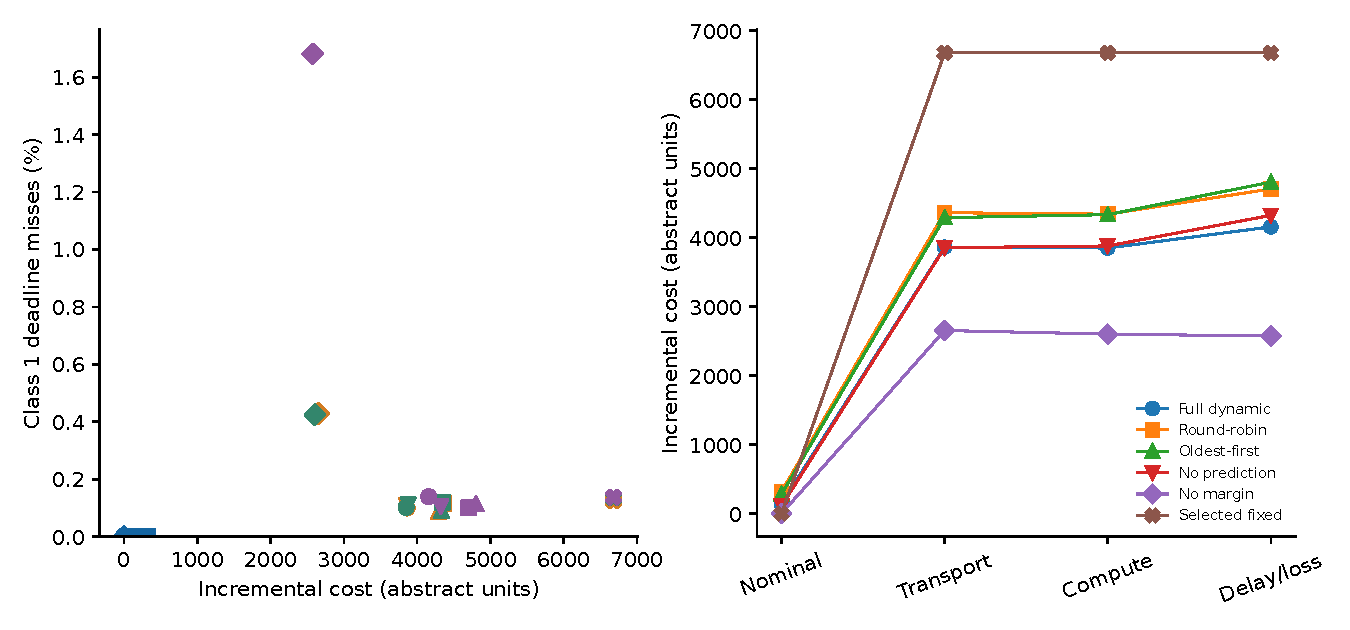
\includegraphics[width=\textwidth]{ablation.pdf}\par
\textbf{Figure 1.} Cost and deadline outcomes across all variants. Scatter colors
identify nominal (blue), transport (orange), compute (green) and delayed/lost
reports (purple). Marker shapes identify methods, as in the right-panel legend.
Both panels are descriptive seed means. The numeric table on the preceding page
includes both classes and avoids hiding small class-0 rates.

\textbf{Margin trade-off.} Removing the margin substantially reduces resource cost
but raises misses under stress. It removes needless nominal expansion in this
sample. This supports a conservatism trade-off, not a calibrated reliability guarantee.

\textbf{Prediction is not uniformly beneficial.} Under delayed/lost reports,
removing extrapolation lowers the observed class-1 miss rate at higher cost.
Under ordinary transport stress it slightly lowers cost while increasing misses.
The present evidence does not justify saying that prediction improves every case.

\textbf{Telemetry priority is not universally dominant.} Round-robin and
oldest-first cost more in the stressed settings, but can have lower class-1 miss
rates. In the delayed/lost setting they also show small class-0 misses absent in
the full variant. The two-class trade-off must remain visible.

\textbf{Nominal overhead.} Fixed zero expansion attains the same observed zero
misses as full dynamic with no extra resource cost. Relative savings against a
zero-cost comparator are undefined, not 0\% or 100\%. This failure case should
inform any future redesign, which must be tested on a new evaluation set.

\page{Activation-delay sensitivity}
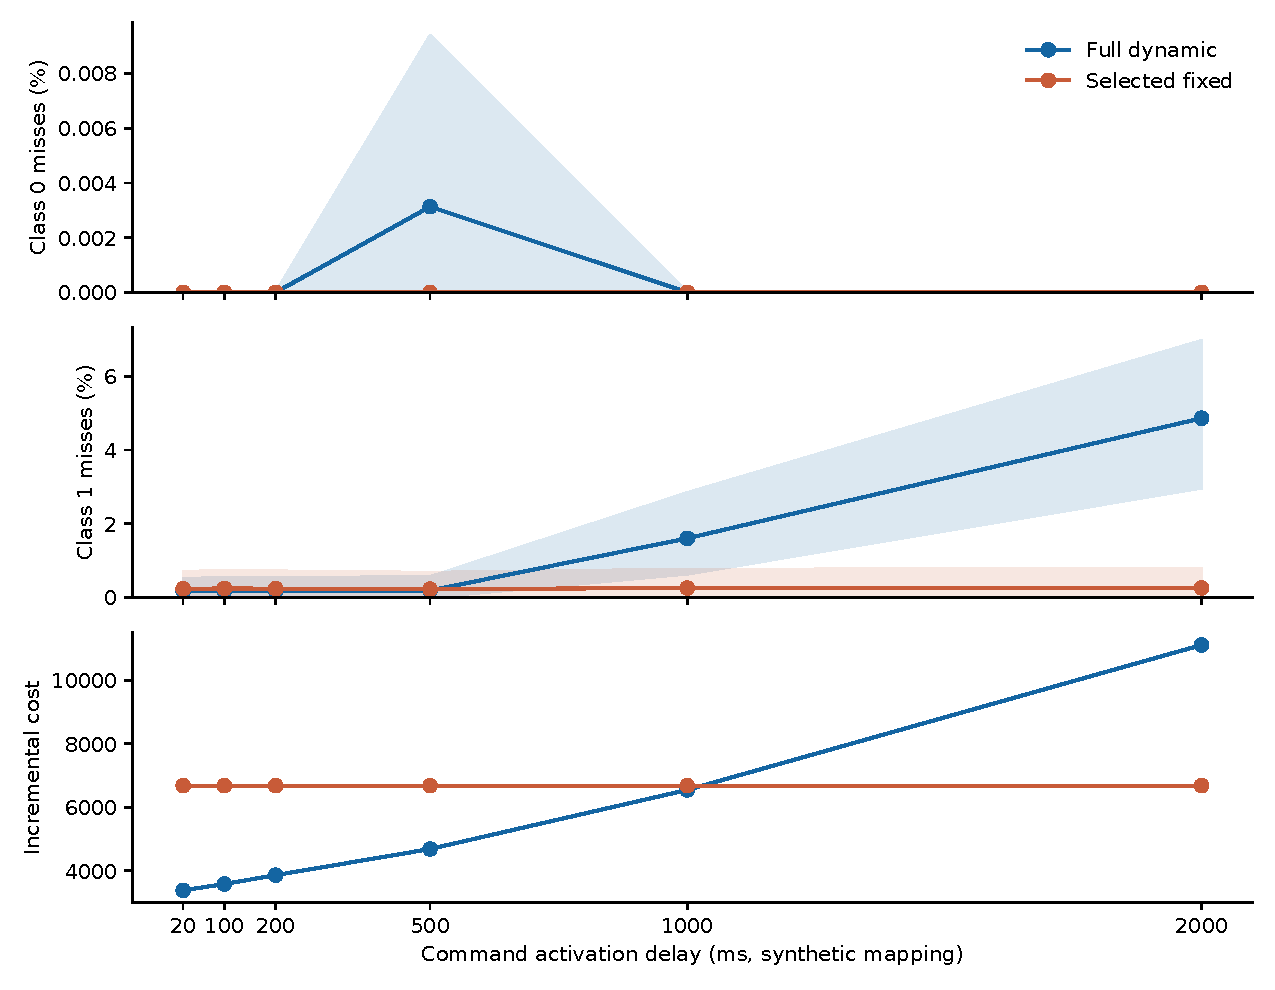
\includegraphics[width=\textwidth,height=110mm,keepaspectratio]{activation_delay.pdf}\par
\textbf{Figure 2.} Transport stress with report delay 3 slots and loss 0.05.
Shading shows exploratory 95\% seed-bootstrap intervals for miss rates. Ten seeds
per point are separate from the primary replication. Fixed expansion is
preprovisioned, but its share updates retain the same command delay.

\begin{center}\scriptsize
\begin{tabular}{rlrrr}\toprule
Delay (ms) & Variant & Class 0 (\%) & Class 1 (\%) & Cost\\\midrule
20 & Full dynamic & 0.0000 & 0.1715 & 3379.07 \\
20 & Selected fixed & 0.0000 & 0.2359 & 6680.00 \\
100 & Full dynamic & 0.0000 & 0.1811 & 3577.88 \\
100 & Selected fixed & 0.0000 & 0.2442 & 6680.00 \\
200 & Full dynamic & 0.0000 & 0.1811 & 3857.35 \\
200 & Selected fixed & 0.0000 & 0.2401 & 6680.00 \\
500 & Full dynamic & 0.0031 & 0.1879 & 4681.50 \\
500 & Selected fixed & 0.0000 & 0.2277 & 6680.00 \\
1000 & Full dynamic & 0.0000 & 1.6042 & 6545.60 \\
1000 & Selected fixed & 0.0000 & 0.2565 & 6680.00 \\
2000 & Full dynamic & 0.0000 & 4.8641 & 11116.77 \\
2000 & Selected fixed & 0.0000 & 0.2593 & 6680.00 \\
\bottomrule\end{tabular}\end{center}
The delay sweep is an exploratory stress test, not measured RIC/SDN or cloud
activation latency. Pending commands are applied in order rather than superseded.
At 2 s, dynamic class-1 misses are 4.8641\% versus 0.2593\% for fixed expansion,
while costs are 11116.78 versus 6680.00. This is a clear failure region of the
present design, not an outlier to remove. It motivates pending-command-aware
control and a new independent evaluation after any redesign.

\page{Paired uncertainty, tests and verification}
Differences are full dynamic minus selected fixed. Negative cost means lower
incremental cost. Class differences are percentage points (pp). Confidence
intervals concern seed-mean differences. Holm p-values concern paired direction,
not the same estimand as a mean-difference test.
\begin{center}\scriptsize
\begin{tabular}{llrrr}\toprule
Setting & Endpoint & Difference & 95\% bootstrap interval & Holm p\\\midrule
Nominal & Class 0 (pp) & 0.0000 & [0.0000, 0.0000] & 1.000 \\
Nominal & Class 1 (pp) & 0.0000 & [0.0000, 0.0000] & 1.000 \\
Nominal & Cost & 142.3125 & [119.8747, 165.6144] & 0.000023 \\
Transport stress & Class 0 (pp) & 0.0000 & [0.0000, 0.0000] & 1.000 \\
Transport stress & Class 1 (pp) & -0.0251 & [-0.0754, 0.0000] & 1.000 \\
Transport stress & Cost & -2816.4000 & [-2890.7250, -2741.5741] & 0.000023 \\
Compute stress & Class 0 (pp) & 0.0000 & [0.0000, 0.0000] & 1.000 \\
Compute stress & Class 1 (pp) & -0.0326 & [-0.0978, 0.0000] & 1.000 \\
Compute stress & Cost & -2829.3875 & [-2906.1250, -2744.0103] & 0.000023 \\
Delayed/lost reports & Class 0 (pp) & 0.0000 & [0.0000, 0.0000] & 1.000 \\
Delayed/lost reports & Class 1 (pp) & 0.0022 & [-0.1243, 0.1310] & 1.000 \\
Delayed/lost reports & Cost & -2523.0125 & [-2613.8394, -2425.0434] & 0.000023 \\
\bottomrule\end{tabular}\end{center}
Intervals that include zero do not establish equivalence. All-zero bootstrap
intervals do not prove zero population risk. No noninferiority margin was
specified, so no noninferiority claim is made.

\subsection*{Independent software verification}
The packet reference uses simultaneous outgoing lists and birth-time FIFO queues,
whereas the production model uses downstream-first deque updates. Across 18
scenario/policy checks, arrivals, late completions, unfinished packets, miss
rates, backlog and completed-delay percentiles agree exactly. This reference
replays applied actions, so it validates the data plane conditional on those
actions, not the whole controller implementation.

An independently written, uncached optimizer checks 30 random report states
against the cached implementation. Chosen expansions/shares agree, and numerical
ratios agree to 12 decimal places. Separate tests cover deadline boundaries,
zero load, zero capacity, future-trace noninterference and invalid delays.
The complete suite has 37 passing unit-test methods. Six regression comparisons
confirm unchanged default behavior against the prior engine.

Whole-output validation checks all 600 new records, the locked protocol hash,
seed separation, report budgets, cost identities, capacity limits, measured-cohort
rates and the 12-test Holm adjustment. These are software checks, not physical
model validation. Raw records and scripts are included in the reproducibility archive.

\page{Publication gate and next experiment}
IEEE TNSM explicitly welcomes theoretical and applied network/service-management
contributions \cite{tnsm}. Thus hardware is not universally mandatory. However,
neither scope fit nor clean formatting establishes originality or acceptance.
Current journal quartiles were not verified in this study.

\begin{center}\small
\begin{tabular}{p{36mm}p{48mm}p{65mm}}\toprule
Requirement & Current state & Evidence still required\\\midrule
Mathematical model & Explicit and matched to code & Substantial new result beyond finite-grid correctness\\
Software verification & 37 tests and independent checks & Broader scale/topology validation after model extension\\
Physical calibration & Not available & Radio/link/CPU model with documented units and provenance\\
External validation & Not executed & Calibrated network simulator or independent measured traces\\
Published baselines & Context reviewed, not reproduced & Faithful compatible implementations and matched assumptions\\
Literature depth & 13 focused sources & Complete closest-work review, including the requested 40 relevant references\\
Three-paper program & One abstract model only & Distinct controllers/questions and separate evidence for each paper\\\bottomrule
\end{tabular}\end{center}

\textbf{Required source inputs.} The approved proposal and the student's current
simulator/configuration or measured traces are needed to align a physical study
with the thesis. If none exists, a deployment scenario must be selected for a
calibrated system-level simulator. Necessary fields include bandwidth, channel,
topology, users, payload sizes, transport links, compute workload, deadlines,
telemetry overhead and resource activation mechanisms.

\textbf{Proposed next validation, not completed work.} Pin a documented external
calibration case and reproduce its reference metrics first. Define acceptable
differences before viewing outputs. Introduce the controller without changing
the calibrated data-plane defaults. Reproduce the closest compatible published
baseline, freeze fresh test traces, and report all differences and failure cases.

\textbf{Three-paper separation.} A telemetry/elasticity paper needs stronger
novelty and validation. An asynchronous-control paper needs a pending-action-aware
controller and a new safety/feasibility result. A recovery paper needs explicit
failures, recovery actions and recovery-time constraints. The present burst tests
do not constitute a fault-recovery experiment.

\textbf{Conclusion.} The artifact establishes a reproducible synthetic trade-off
between paid capacity, delayed information and deadline misses. It also identifies
negative outcomes and uncontrolled assumptions. These results are sufficient for
technical review and model development, not for claiming completed Q1-ready O-RAN papers.

\clearpage
\begin{thebibliography}{13}\small
\bibitem{polese} M. Polese, L. Bonati, S. D'Oro, S. Basagni and T. Melodia,
``Understanding O-RAN: Architecture, Interfaces, Algorithms, Security, and Research Challenges,''
arXiv:2202.01032v2, 2022. \url{https://arxiv.org/abs/2202.01032}.
\bibitem{age} R. D. Yates, Y. Sun, D. R. Brown III, S. K. Kaul, E. Modiano and S. Ulukus,
``Age of Information: An Introduction and Survey,'' arXiv:2007.08564, 2020.
\url{https://arxiv.org/abs/2007.08564}.
\bibitem{marea} O. Adamuz-Hinojosa, L. Zanzi, V. Sciancalepore and X. Costa-Perez,
``MAREA: A Delay-Aware Multi-time-Scale Radio Resource Orchestrator for 6G O-RAN,''
IEEE Transactions on Communications, 2025. \url{https://doi.org/10.1109/TCOMM.2025.3552296}.
Author text: \url{https://arxiv.org/html/2503.08599v2}.
\bibitem{kalntis} M. Kalntis, G. Iosifidis and F. A. Kuipers,
``Adaptive Resource Allocation for Virtualized Base Stations in O-RAN With Online Learning,''
IEEE Transactions on Communications. \url{https://doi.org/10.1109/TCOMM.2024.3461569}.
Author text: \url{https://arxiv.org/html/2309.01730v2}.
\bibitem{demir} O. T. Demir, M. Masoudi, E. Bjornson and C. Cavdar,
``Cell-Free Massive MIMO in O-RAN: Energy-Aware Joint Orchestration of Cloud, Fronthaul, and Radio Resources,''
IEEE JSAC, vol. 42, no. 2, pp. 356--372, 2024. \url{https://doi.org/10.1109/JSAC.2023.3336187}.
\bibitem{oreo} F. Mungari, C. Puligheddu, A. Garcia-Saavedra and C. F. Chiasserini,
``OREO: O-RAN intElligence Orchestration of xApp-based network services,''
arXiv:2405.18198v2, 2024. \url{https://arxiv.org/abs/2405.18198}.
\bibitem{caora} S. D. A. Shah, M. Hafeez, A. Salama and S. A. R. Zaidi,
``Proactive AI-and-RAN Workload Orchestration in O-RAN Architectures for 6G Networks,''
arXiv:2507.09124, 2025. \url{https://arxiv.org/abs/2507.09124}.
\bibitem{coloran} M. Polese, L. Bonati, S. D'Oro, S. Basagni and T. Melodia,
``ColO-RAN: Developing Machine Learning-based xApps for Open RAN Closed-loop Control on Programmable Experimental Platforms,''
arXiv:2112.09559v2, 2022. \url{https://arxiv.org/abs/2112.09559}.
\bibitem{lena} N. Patriciello, S. Lagen, B. Bojovic and L. Giupponi,
``An E2E Simulator for 5G NR Networks,'' Simulation Modelling Practice and Theory,
vol. 96, article 101933, 2019. Developer bibliography: \url{https://5g-lena.cttc.es/papers/}.
\bibitem{calibration} K. Koutlia, B. Bojovic, Z. Ali and S. Lagen,
``Calibration of the 5G-LENA System Level Simulator in 3GPP reference scenarios,''
Simulation Modelling Practice and Theory, vol. 119, article 102580, 2022.
\url{https://5g-lena.cttc.es/features/calibration/}.
\bibitem{efron} B. Efron, ``Bootstrap Methods: Another Look at the Jackknife,''
The Annals of Statistics, vol. 7, no. 1, pp. 1--26, 1979.
\url{https://doi.org/10.1214/aos/1176344552}.
\bibitem{holm} S. Holm, ``A Simple Sequentially Rejective Multiple Test Procedure,''
Scandinavian Journal of Statistics, vol. 6, pp. 65--70, 1979.
\url{https://www.jstor.org/stable/4615733}.
\bibitem{tnsm} IEEE Communications Society, ``IEEE Transactions on Network and Service Management,''
official journal scope, accessed 18 October 2026.
\url{https://www.comsoc.org/publications/journals/ieee-transactions-network-and-service-management}.
\end{thebibliography}
\textbf{Source audit.} Author abstracts/metadata were checked for [1], [2], [5]--[8].
Full-text sections and identifiers were checked for [3], [4]. Official developer
documentation supports [9], [10]. [11], [12] are method attributions with limited
archive access, not a claim of full-text review. [13] is the official journal page.
The detailed source ledger is supplied in SOURCE\_AUDIT.md. No bibliography-size
or comprehensive-novelty claim is made.
\end{document}
